\documentclass[12pt]{article}
\usepackage[english]{babel}
\usepackage[utf8]{inputenc}
\usepackage{amsmath, amssymb, amsthm}
\usepackage{graphicx}
\usepackage{hyperref}
\usepackage[margin=.75in]{geometry}
\usepackage{xcolor}
\usepackage{tikz}

\newcommand{\id}{\text{id}}
\newcommand{\od}{\text{od}}

\setlength{\topmargin}{0pt}
\setlength{\headsep}{0pt}
\textheight = 600pt

\title{Graph Theory \\ Homework 18}
\author{Ben Kallus and Josef Komissar}
\date{Due Monday, May 10}

\begin{document}

\maketitle

\medskip\noindent\textbf{11.6} $r(K_{1, 3}, P_3) = 5$.
\begin{proof}
    Note that $r(K_{1, 3}, P_3) > 4$ because of the following counterexample:

    \begin{center} 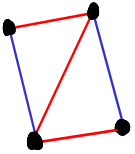
\includegraphics{1.png} \end{center}

    We now show that $r(K_{1, 3}, P_3) \leq 5$.
    Color the edges of $K_5$ red and blue.
    Suppose some vertex has two or more blue incident edges.
    Then the graph has a blue $P_3$ as a subgraph.
    If no vertex has two or more blue incident edges, then some vertex $v$ has less than two blue incident edges.
    Thus, $v$ must have at least three incident red edges, which creates a red claw as a subgraph.

    Thus, $r(K_{1, 3}, P_3) = 5$.
\end{proof}

\newpage\noindent\textbf{11.8} $r(2K_2, 3K_2) = 6$.
\begin{proof}
    Note that for any complete graph or order less than 6, we can color every edge blue and not create a $3K_2$ subgraph.
    Obviously, such a graph would not have a red $2K_2$ subgraph, so $r(2K_2, 3K_2) \geq 6$.
    
    We now show that $r(2K_2, 3K_2) \leq 6$.
    Color the edges of $K_6$ blue and red.
    If any two independent edges are red, then the graph has a red $2K_2$ subgraph.
    Suppose that no two independent edges are red.
    Then, the graph has either all blue edges, exactly one red edge, exactly two red edges, which are adjacent, or exactly three red edges that form a triangle.
    Obviously, if the graph has no red edges, then it contains a blue $3K_2$ subgraph.
    If the graph contains only a single red edge, then because all edges in $K_6$ are symmetric, the following drawing shows that the graph contains a blue $3K_2$ subgraph:
    \begin{center} 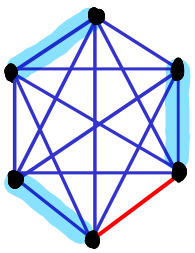
\includegraphics[scale=.5]{2.png} \end{center}
    If the graph contains two adjacent red edges, then because all pairs of adjacent edges in $K_6$ are symmetric, the following drawing shows that the graph contains a blue $3K_2$ subgraph:
    \begin{center} 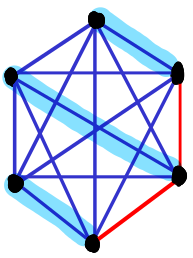
\includegraphics[scale=.5]{3.png} \end{center}
    If the graph contains a red triangle, then because all triangles in $K_6$ are symmetric, the following drawing shows that the graph contains a blue $3K_2$ subgraph:
    \begin{center} 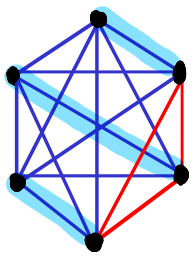
\includegraphics[scale=.5]{4.png} \end{center}
    Thus, $r(2K_2, 3K_2) \leq 6$, so $r(2K_2, 3K_2) = 6$.
\end{proof}

\newpage\noindent\textbf{11.10} $r(P_3, P_3 \cup P_2) = 5$.
\begin{proof}
    Note that $r(P_3, P_3 \cup P_2) > 4$ because of the following counterexample:

    \begin{center} 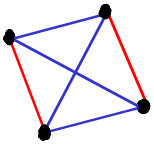
\includegraphics{5.png} \end{center}

    We now show that $r(P_3, P_3 \cup P_2) \leq 5$.
    Color the edges of $K_5$ blue and red.
    If there is only one red edge, the because all edges in a complete graph are symmetric, the image below shows that the graph has a blue $P_3\cup P_2$ subgraph.
    \begin{center} 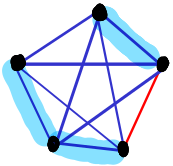
\includegraphics{6.png} \end{center}
    If there are exactly two nonadjacent red edges, then because every pair of nonadjacent edges in a complete graph is symmetric, there is a blue $P_3\cup P_2$ subgraph as seen in the image below:
    \begin{center} 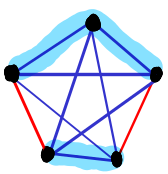
\includegraphics{7.png} \end{center}
    If there are three or more red edges, two of them must be adjacent by the Pigeonhole principle, so the graph contains a red $P_3$ subgraph.
    Thus, $r(P_3, P_3 \cup P_2) = 5$.
\end{proof}

\newpage\noindent\textbf{11.12} $r(P_4, P_4) = 5$.
\begin{proof}
    The following counterexample shows that $r(P_4, P_4) > 4$:
    \begin{center} 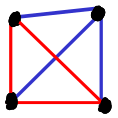
\includegraphics{8.png} \end{center}
    
        We now show that $r(P_4, P_4) \leq 5$.
        Color the edges of $K_5$ red and blue.
        Suppose that there is a vertex $v$ with neighbors $u, w, x$ all connected to $v$ by red edges.
        Suppose without loss of generality that $u$ and $w$ are connected by a red edge.
        Then, the graph contains the red $P_4$ induced by $\{u, w, v, x\}$.
        By a symmetric argument, if there is a vertex with three or more incident blue edges, then the graph contains a blue $P_4$.
        Suppose that every vertex in the graph is incident to exactly 2 red edges and 2 blue edges.
        Note that the construction of any such graph would begin with a graph isomorphic to the one shown below:
        \begin{center} 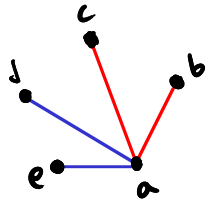
\includegraphics[scale=.7]{9.png} \end{center}
        No matter the color of the edge $bd$, a monochromatic $P_4$ will be created.
        Thus, $r(P_4, P_4) = 5$.
\end{proof}

\newpage\noindent\textbf{11.16} $r(K_3, K_n) \leq {n+1 \choose 2}$ for all $n \geq 2$.
\begin{proof}
    Observe that $r(K_3, K_2) = \max\{|V(K_3)|, |V(K_2)|\} = 3$.
    Suppose that $r(K_3, K_{n-1}) \leq {n \choose 2}$ for some $n \geq 3$.
    

\end{proof}

\newpage\noindent\textbf{LASTLY} The Book is Erdös's hypothetical transfinite book containing all the best possible proofs that are ``elegant and perfect."

\end{document}

